%%%%%%%%%%%%%%%%%%%%%%%%%%%%%%%%%%%%%%%%%%%%%%%%%%%%%%%%%%%%%%%%%%%%%%%%%%%%% 
%
% This is a LaTeX file for an A0 poster.
% 
% template poster taken from https://canizo.org/latex_poster
%
%%%%%%%%%%%%%%%%%%%%%%%%%%%%%%%%%%%%%%%%%%%%%%%%%%%%%%%%%%%%%%%%%%%%%%%%%%%%% 

%%%%%%%%%%%%%%%%%%%%%%%%%%%%%%%%%%%%%%%%%%%%%%%%%%%%%%%%%%%%%%%%%%%%%%%%%%%%% 
%%%%%%%%%%%%%%%%%%%%%%%%%%%%%%%%%%%%%%%%%%%%%%%%%%%%%%%%%%%%%%%%%%%%%%%%%%%%%
%
% scpdata: a data package for single-cell proteomics
%
% Poster for the Eurobioc2019, December 2019.
%
%%%%%%%%%%%%%%%%%%%%%%%%%%%%%%%%%%%%%%%%%%%%%%%%%%%%%%%%%%%%%%%%%%%%%%%%%%%%%
%%%%%%%%%%%%%%%%%%%%%%%%%%%%%%%%%%%%%%%%%%%%%%%%%%%%%%%%%%%%%%%%%%%%%%%%%%%%%

\documentclass{article}
% To modify the size of the page:
\usepackage[dvips,a3paper,portrait,centering,margin=0.4cm]{geometry}
% To create multiple columns
\usepackage{multicol}

\usepackage[utf8]{inputenc}
% To align images
\usepackage[export]{adjustbox}
% Use captions in minipages
\usepackage{caption}
% Math font
\usepackage{amsmath, amsthm, amsfonts}
% Include figure files.
\usepackage{graphicx}

% Coding fonts
% ------------
% For including R chunks 
\usepackage{listings} 
\lstset{language=R,
language=R,                     % the language of the code
  basicstyle=\footnotesize,       % the size of the fonts that are used for the code
  numbers=left,                   % where to put the line-numbers
  numberstyle=\tiny\color{gray},  % the style that is used for the line-numbers
  stepnumber=1,                   % the step between two line-numbers. If it's 1, each line
                                  % will be numbered
  numbersep=5pt,                  % how far the line-numbers are from the code
  backgroundcolor=\color{white},  % choose the background color. You must add \usepackage{color}
  showspaces=false,               % show spaces adding particular underscores
  showstringspaces=false,         % underline spaces within strings
  showtabs=false,                 % show tabs within strings adding particular underscores
  frame=single,                   % adds a frame around the code
  rulecolor=\color{black},        % if not set, the frame-color may be changed on line-breaks within not-black text (e.g. commens (green here))
  tabsize=2,                      % sets default tabsize to 2 spaces
  captionpos=b,                   % sets the caption-position to bottom
  breaklines=true,                % sets automatic line breaking
  breakatwhitespace=false,        % sets if automatic breaks should only happen at whitespace
  title=\lstname,                 % show the filename of files included with \lstinputlisting;
                                  % also try caption instead of title
  keywordstyle=\color{blue},      % keyword style
  commentstyle=\color{dkgreen},   % comment style
  stringstyle=\color{mauve},      % string literal style
  escapeinside={\%*}{*)},         % if you want to add a comment within your code
  morekeywords={*,...             % if you want to add more keywords to the set
    % basicstyle=\small\ttfamily\color{vdgray},
    % stringstyle=\color{green},
    % keywordstyle=\color{blue},
    % deletekeywords={},
    % breakatwhitespace=false,
    % morekeywords={}
}
% Create command for highlighting inline code or variables
\newcommand{\hcode}[2][lgray]{{\ttfamily\color{vdgray}\colorbox{#1}{#2}}}

% Colors
% ------
\usepackage{color}
\usepackage[dvipsnames]{xcolor}
% Color panel used throughout the poster
\definecolor{lgray}{rgb}{0.9179688,0.9179688,0.9179688}
\definecolor{dgray}{rgb}{0.796875,0.796875,0.796875}
\definecolor{vdgray}{rgb}{0.3984375,0.3984375,0.3984375}
\definecolor{coral}{rgb}{0.9960938,0.4960938,0.3125000}
\definecolor{blue}{rgb}{0.4218750,0.6484375,0.8007812}
\definecolor{green}{rgb}{0.6992188,0.7265625,0.5078125}
\definecolor{yellow}{rgb}{0.9570312,0.8671875,0.6992188}

% Adjust space between reference items
% ------------------------------------
\let\OLDthebibliography\thebibliography
\renewcommand\thebibliography[1]{
  \OLDthebibliography{#1}
  \setlength{\parskip}{0pt}
  \setlength{\itemsep}{0pt plus 0.3ex}
}
  
\pagestyle{empty}

\def\to{\rightarrow}


% ===========================================================================

\title{}
\author{}
\date{}

\begin{document}


% ---------------------------------------------------------------------------
% Banner


\begin{center}
\fcolorbox{lgray}{lgray}{
  \begin{minipage}{3cm}
    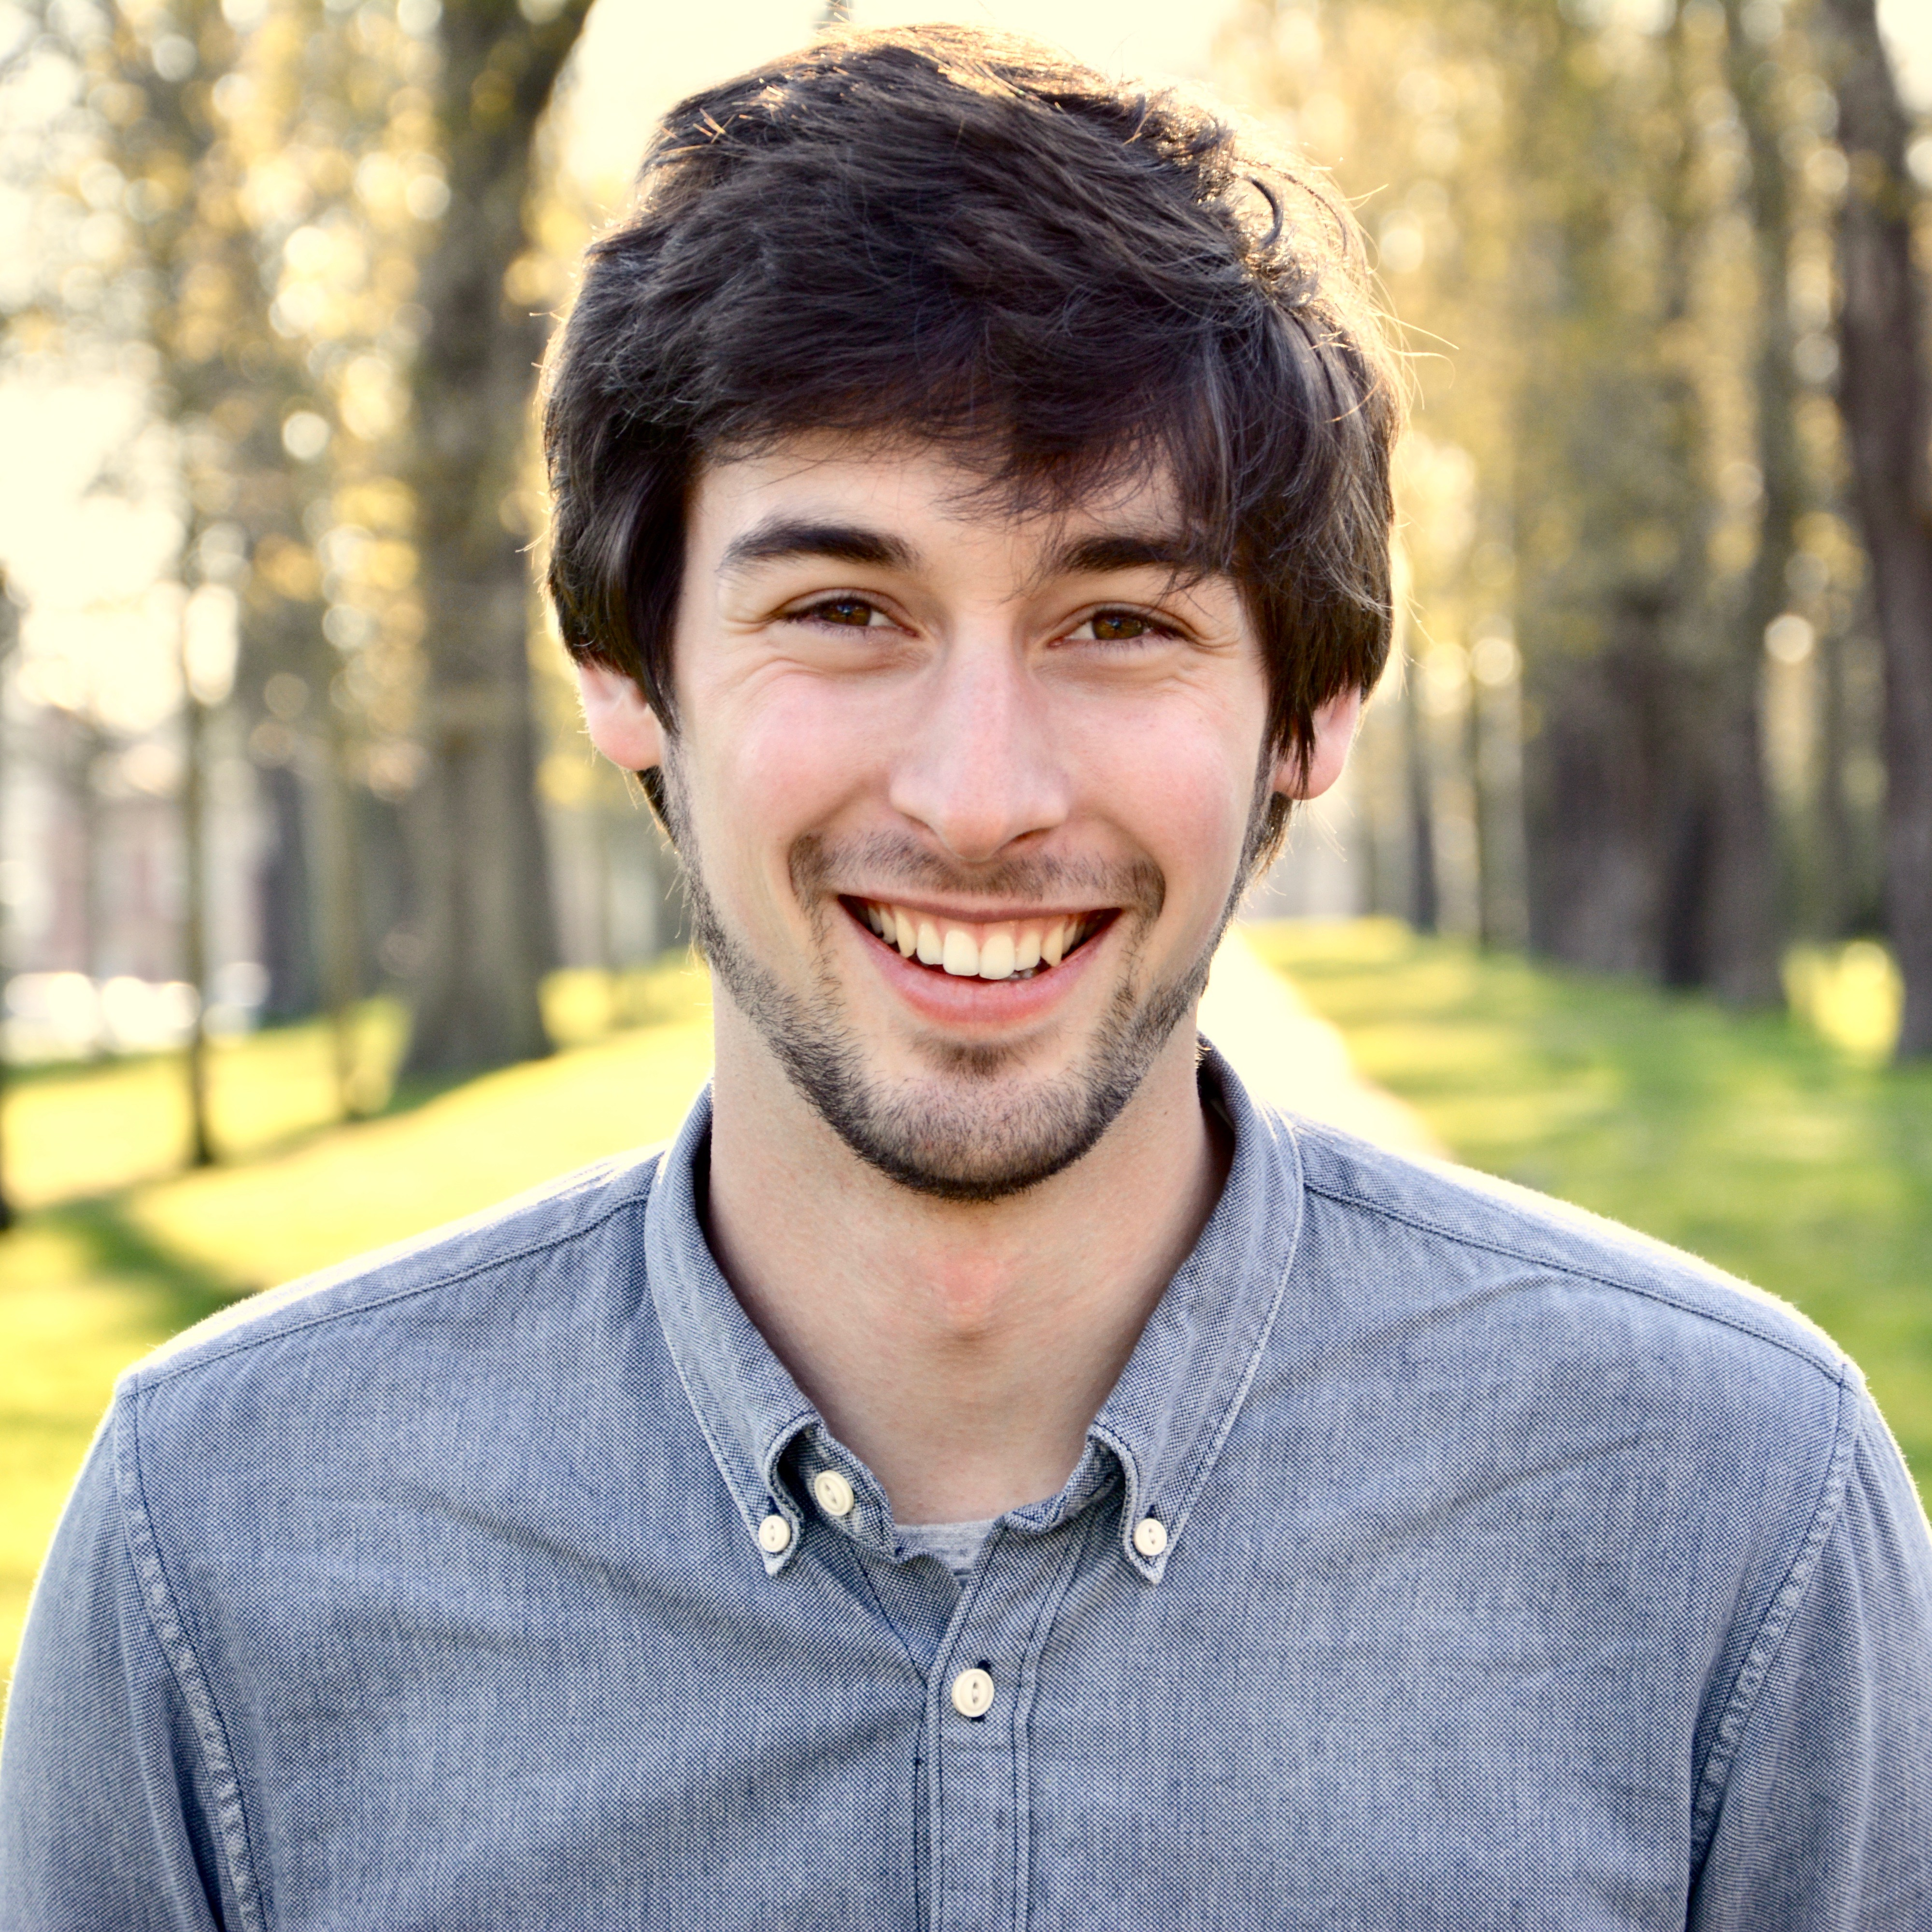
\includegraphics[width=1.2\linewidth]{figs/DSC_2812.jpg}
  \end{minipage}
  %&
  \begin{minipage}{.74\textwidth}
    \begin{center}
      % Title 
      \huge \textbf{scpdata: a data package for single-cell proteomics} \\
      \vspace{0.4cm}
      % Authors
      \Large \textbf{Christophe Vanderaa, Laurent Gatto} \\
      % Affiliation
      \Large \textit{Computational biology and bioinformatics lab, de Duve Institute, UCLouvain } \\
      % email
      \vspace{0.4cm}
      \normalsize christophe.vanderaa@uclouvain.be \\
    \end{center}
  \end{minipage}
  %&
  \begin{minipage}{3.7cm}
      \includegraphics[width=0.7\linewidth, right]{figs/fnrs.png} \\
      \vspace{0.5cm}
      \includegraphics[width=1.1\linewidth, right]{figs/ucl.png}
  \end{minipage}
}
\end{center}


% ------------------------\---------------------------------------------------
% Summary

\setlength{\columnsep}{1cm}
\begin{multicols}{2}

\noindent
\fcolorbox{yellow}{yellow}{
  \begin{minipage}[t]{\linewidth}
      \vspace{.15cm}
      \section*{\huge Summary}
      \large Recent advances in sample preparation, processing and mass spectrometry (MS) have allowed the emergence of MS-based single-cell proteomics (SCP). However, bioinformatics tools to process and analyze these new types of data are still missing. In order to boost the development and the benchmarking of SCP methodologies, we are developing the \hcode[yellow]{scpdata} experiment package. The package will distribute published and curated SCP data sets in standardized Bioconductor format. 
    
  \end{minipage}
}
\noindent

% ---------------------------------------------------------------------------
% Introduction
\noindent
\begin{minipage}[t]{\linewidth}
  \vspace{0.55cm}
  \section*{\huge Introduction}
  \large
  
  There are two main pipelines able to generate MS-SCP data:

  \begin{itemize}
    \item \textbf{\large nanoPOTS pipeline} (Zhu et al., 2018, \cite{Zhu2018-bf}) runs label-free proteomics for single cells. The \textbf{\color{BrickRed}{throughput is low}} ($\pm$ 10 samples/day), but achieves \textbf{\color{OliveGreen}{accurate peptide quantification}}. 
  
  \begin{center}
    % \includegraphics[width=\linewidth]{figs/nanoPOTS.png} \\
  \end{center}
        
    \item \textbf{\large SCoPE pipeline} (Slavov Lab, 2018, \cite{Budnik2018-qh}) adapts TMT-based proteomics to single-cells. The \textbf{\color{OliveGreen}{throughput is higher}} ($\pm$ 5 samples/hour) and the identification rate, but \textbf{\color{BrickRed}{presence of chemical noise}}.
  \end{itemize}
  
  \begin{center}
    % \includegraphics[width=0.5\linewidth]{figs/scopems.png} \\
  \end{center}
  
\end{minipage}

% ---------------------------------------------------------------------------
% Content of the package
\noindent
\begin{minipage}[t]{\linewidth}
  \vspace{0.55cm}
  \section*{\huge Content of the package}
  
  \large
  \hcode{scpdata} contains SCP data sets formatted as \hcode{MSnbase::MSnSet} objects. The package provides data at \textbf{peptide} and \textbf{protein} level. \textbf{Help files} are provided for every data set and accessed using \hcode{?dou2019\_1\_protein}. Available data sets are listed using \hcode{scpdata()}.
  
  \scriptsize
  \begin{tabular}{@{\extracolsep{5pt}} cl} 
    \\[-1.8ex]\hline 
    \hline \\[-1.8ex] 
    \textbf{Item} & \textbf{Title} \\ 
    \hline \\[-1.8ex] 
    dou2019\_1\_protein & FACS + nanoPOTS + TMT multiplexing: HeLa digests (Dou et al. 2019) \\ 
    dou2019\_2\_protein & FACS + nanoPOTS + TMT multiplexing: testing boosting ratios (Dou et al. 2019) \\ 
    dou2019\_3\_protein & FACS + nanoPOTS + TMT multiplexing: profiling of murine cell populations (Dou... \\
    specht2018\_peptide & SCoPE-MS + mPOP lysis upgrade: Master Mix 20180824 (Specht et al. 2018) \\ 
    specht2019\_peptide & FACS + SCoPE2: comparing macrophages against monocytes (Specht et al. 2019) \\ 
    specht2019\_peptide2 & FACS + SCoPE2: comparing macrophages against monocytes (Specht et al. 2019) \\ 
    specht2019\_protein & FACS + SCoPE2: comparing macrophages against monocytes (Specht et al. 2019) \\ 
    \hline \\[-1.8ex] 
  \end{tabular} 
  
\end{minipage}
  

% ---------------------------------------------------------------------------
% Data manipulation
\noindent
\begin{minipage}[t]{\linewidth}
  \vspace{0.55cm}
  \section*{\huge Data manipulation}
  \large
  
  The Bioconductor class \hcode{MSnSet} is a reliable framework for standard and systematic data processing. Below, the re-implementation of the R script provided in \cite{Specht2019-jm}:
  
  \begin{lstlisting}[backgroundcolor=\color{lgray}, language=R]
    data("specht2019_peptide")
    specht2019_peptide %>% 
      scp_normalize_stat(what = "row", mean, "-") %>%
      scp_aggregateByProtein() %>%
      scp_normalize_stat(what = "column", median, "-") %>%
      scp_normalize_stat(what = "row", mean, "-") %>%
      imputeKNN(k = 3) %>%
      batchCorrect(batch = "raw.file", target = "celltype") -> scpd
  \end{lstlisting}
  
    
\end{minipage}

% ---------------------------------------------------------------------------
% Data quality control
\noindent
\begin{minipage}[t]{\linewidth}
  \vspace{0.55cm}
  \section*{\huge Data quality control}
  \large
  
  When developing the SCoPE technology, the Slavov lab also suggested some quality control (QC) measures and visualizations \cite{Huffman2019-ns} (eg Figure \ref{fig:qc}). The \hcode{scpdata} package provides an ideal data environment for developing and improving SCP data QC.
  
    \centering
      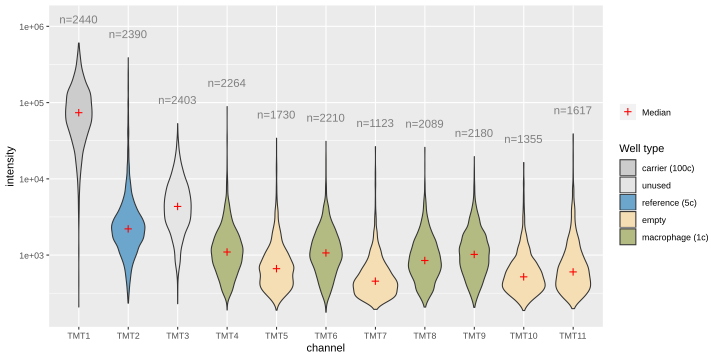
\includegraphics[width=\textwidth]{figs/QC.png}
   \captionof{figure}{\textbf{MS intensity distributions per channel at peptide level.} \small Contamination peptides or peptides with a low identification score were removed. Data taken from run \hcode{190222S\_LCA9\_X\_FP94BF} published in \cite{Specht2019-jm}. n: number of non-missing peptides.}
   \label{fig:qc}
  
\end{minipage}



% ---------------------------------------------------------------------------
% Data benchmarking
\noindent
\begin{minipage}[t]{\linewidth}
  \vspace{0.55cm}
  \section*{\huge Data benchmarking}
  \large
  
  \hcode{scpdata} also offers an ideal environment for benchmarking. 
  Th  ere are 2 mindsets for data validation:
  
  - Generate in vitro/silico simulated data sets: ground truth is known but could deviate from reality
  - Generate data from biological samples with some prior knowledge : close to a real experiment but no ground truth available
  
  Dimension reduction and data visualization (PCA, tSNE, UMAP) is often used for validating data (Figure \ref{fig:pca}). When phenotype information is available, objective benchmarking metrics can be used: silhouette width, entropy of cluster accuracy, kBET for batch correction. 

  \centering
    
\includegraphics[width=\textwidth]{figs/PCA.png}
  \captionof{figure}{\textbf{PCA plot of peptide expression data.} \small Macrophages and monocytes are well separated in the third principal component. However, the first and second components are driven by batch effects. Monocytes are untreated U-937 cells, macrophages are U-937 treated with PMA for 24 hours. LCA10 and LCA9 are two chromatographic batches. The PCA was performed using the non-linear iterative partial least squares (NIPALS) algorithm that is robust against missing data.}
  \label{fig:pca}

\end{minipage}

% ---------------------------------------------------------------------------
% Problems to tackle: batch effect
\noindent
\begin{minipage}[t]{\linewidth}
  \vspace{0.55cm}
  \section*{\huge Problems to tackle}
  \subsection*{Batch effects}
  \large
  Batch effects are inherent to MS-SCP data since many samples/cells have to be distributed across different MS runs (even with TMT labeling). This leads to tremendous batch effects (Figure \ref{fig:pca}).
  
\end{minipage}
  
% ---------------------------------------------------------------------------
% Problems to tackle: Missingness
\noindent
\begin{minipage}[h]{0.37\linewidth}
  \subsection*{Missingness}
  \large
  The \cite{Specht2019-jm} data sets contains +/- 75 \% missing data. This needs to be accounted for by the statistical methods used for downstream analyses. Furthermore, conditions can be differentially affected by missingness that could lead to imputation-induced differential expression (Figure \ref{fig:missing}).

\end{minipage}
\hspace{0.4cm}
\begin{minipage}[h]{0.6\linewidth}
  \begin{center}
    \includegraphics[width=\linewidth]{figs/missing.png}
  \end{center}
\end{minipage}

\captionof{figure}{\textbf{Distribution of the proportion missing data in monocytes against macrophages.} \small Color indicates the log2 fold change of {\color{coral}macrophages} over {\color{green}monocytes} relative expression.}
\label{fig:missing}


% ---------------------------------------------------------------------------
% Problems to tackle: Curse of dimensionality
\noindent
\begin{minipage}[t]{\linewidth}
  \subsection*{Curse of dimensionality}
  \large
  The current experiments are producing relatively small data sets (thousands of peptides x hundreds of cells) compared to single-cell transcriptomics. Nevertheless, the rapid growing of MS-SCP techniques will lead to data sets of much higher dimensionality. This is a challenge for both the statistical analyses and the software optimization. Possible solution should be inspired from current achievement in single cell transcriptomics. 
  
\end{minipage}

% ---------------------------------------------------------------------------
% Conclusion
\noindent
\fcolorbox{yellow}{yellow}{
  \begin{minipage}[t]{\linewidth}
    \vspace{.15cm}
    \section*{\huge Conclusion}
    \large 
    MS-based SCP is still at its infancy. However, we hope that developing an MS-SCP data package will provide a strong framework for bioinformatics research. It will support the development of new packages for tackling the statistical issues (missing data, batch effect, high dimensionality) seen in MS-SCP data, as well as providing a growing data repository for software benchmarking. By thorough implementation and benchmarking of its software, MS-SCP might become a new state-of-the-art technique for single-cell omcis.
  \end{minipage}
}


% ---------------------------------------------------------------------------
% References
\scriptsize
\bibliography{ref.bib} 
\bibliographystyle{ieeetr}


\end{multicols}

\end{document}